%!TeX root=../main.tex

\فصل{تشریح پروژه}
\قسمت{مقدمه}
\begin{figure}[!h]
	\centering
	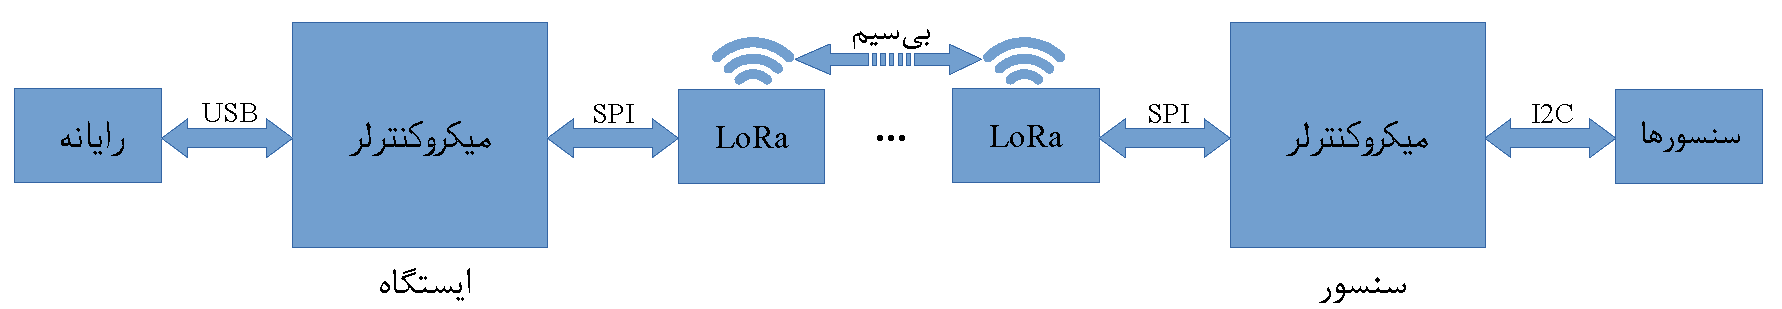
\includegraphics[width=\linewidth]{Assets/system design.pdf}
	\caption{بلوک دیاگرام اجزای سیستم و نحوه ارتباط اجزای مختلف با یکدیگر.}
	\label{fig:systemDesign}
\end{figure}
این سیستم به دو دستگاه اصلی تقسیم می‌شود، یک دستگاه جهت جمع‌آوری اطلاعات جوی برروی یک میله در ارتفاع 10 متری سطح زمین قرار می‌گیرد و اطلاعات جوی نظیر دما، رطوبت، فشار، شدت نور، سرعت و جهت باد را از سنسورهای مربوطه جمع‌آوری کرده و به‌صورت بی‌سیم به دستگاه دیگر، که در ایستگاه اصلی قرار دارد، مخابره می‌کند؛ سپس اطلاعات دریافت شده در سمت دستگاه دوم جهت ثبت و ذخیره به رایانه منتقل می‌شود. در اینجا به دستگاه اول که وظیفه جمع‌آوری اطلاعات جوی را دارد سنسور و دستگاه دوم که وظیفه دریافت اطلاعات مخابره شده و انتقال به رایانه را دارد ایستگاه می‌گوییم. بلوک دیاگرام کلی این سیستم و نحوه ارتباط بخش‌های مختلف با یکدیگر در شکل \رجوع{fig:systemDesign} آمده است.

عملکرد کلی سیستم جمع‌آوری داده‌ها در سمت سنسور، ارسال اطلاعات از طریق لورا به سمت ایستگاه و نمایش اطلاعات دریافت شده در سمت ایستگاه برروی رایانه است. به‌طورکلی این سیستم به دو بخش سنسور و ایستگاه تقسیم می‌شود که بخش ایستگاه خود به دو بخش دستگاه گیرنده و برنامه دسکتاپ (\متن‌لاتین{Desktop}) قابل‌تقسیم است.

\قسمت{سنسور}
فلوچارت فرآیند‌های سمت سنسور در تصویر \رجوع{fig:SensorFlowChart} قابل مشاهده است شرح آن به قرار زیر است:
\شروع{فقرات}
\فقره
بعد از روشن شدن دستگاه و فعالسازی بخش‌های موردنیاز (\متن‌لاتین{peripherals})، میکروکنترلر از طریق \متن‌لاتین{I\بالانویس‌متنی{2}C} با سنسور \متن‌لاتین{BMP180} ارتباط برقرار می‌کند و ضرایب کالیبراسیو را از سنسور \متن‌لاتین{BMP180} می‌خواند این ضرایب برای محاسبه دما و فشار مورداستفاده قرار می‌گیرند \مرجع{sensortec2015digital}.
\فقره
میکروکنترلر با برقراری ارتباط از طریق \متن‌لاتین{I\بالانویس‌متنی{2}C} با سنسور \متن‌لاتین{MAX44009} مقدار رجیستر تنظیمات این سنسور را \متن‌لاتین{0x00} تنظیم می‌کند. در این حالت سنسور در پایین‌ترین سطح مصرف توان خوده قرار می‌گیرد و هر 800 میلی‌ثانیه یکبار میزان شدت نور را اندازه‌گیری می‌کند \مرجع{MAX44009}.
\فقره
با برقراری ارتباطی از طریق \متن‌لاتین{I\بالانویس‌متنی{2}C} با سنسور \متن‌لاتین{HMC5883L} و تنظیم رجیستر تنظیمات، سنسور در حالت آماده‌به‌کار و نرخ نمونه‌برداری 50 هرتز قرار می‌گیرد \مرجع{HMC5883L}.
\فقره
رجیسترهای تنظیمات ماژول \متن‌لاتین{LoRa} با برقراری ارتباط از طریق \متن‌لاتین{SPI} تنظیم‌شده و این ماژول در حالت آماده‌به‌کار قرار می‌گیرد. فرکانس این ماژول روی 433 مگاهرتز، توان آن روی 20 \متن‌لاتین{dBm}، ضریب بخش آن روی 10 و پهنای باند آن روی 31٫2 کیلوهرتز تنظیم می‌گردد (به‌منظور دریافت اطلاعات ارسالی در سمت ایستگاه نیز دقیقاً همین تنظیمات فرکانس، پهنای باند و ضریب پخش باید اعمال شوند) \مرجع{SX1278}.
\فقره
برنامه وارد حلقه اصلی کار خود شده و دما و فشار را با استفاده از سنسور \متن‌لاتین{BMP180} اندازه‌گیری می‌کند. 
\فقره
پس از اندازه‌گیری شدت نور با استفاده از سنسور \متن‌لاتین{MAX44009} \مرجع{MAX44009} و اندازه‌گیری رطوبت هوا به‌وسیله سنسور \متن‌لاتین{AHT10} \مرجع{AHT10}، جهت جغرافیایی توسط سنسور \متن‌لاتین{QMC5883L} \مرجع{HMC5883L} به‌دست می‌آید. 
\فقره
سرعت باد روی دو محور \متن‌لاتین{x} و \متن‌لاتین{y} با استفاده از سنسور \متن‌لاتین{HCSR05} و با توجه به رابطه‌ی \رجوع{eq:speedWindX} محاسبه می‌شود. سپس زاویه و شدت باد با توجه به‌سرعت باد روی هر دو محور با توجه به رابطه \رجوع{eq:windSpeed} به‌دست می‌آید.
\فقره
اطلاعات جمع‌آوری و محاسبه‌شده از طریق ماژول لورا برای گیرنده سمت ایستگاه ارسال می‌شود.
\فقره 
میکروکنترلر و سنسورها در حالت توقف\پانویس{Stop} قرار داده می‌شوند و پس از سه ساعت با رخ‌دادن آلارم\پانویس{Alarm} میکروکنترلر از حالت توقف خارج شده و فرآیند دریافت و ارسال داده‌ها را تکرار می‌کند.
\فقره 
پس از هر بار خارج شدن از حالت توقف، آلارم بعدی برای سه ساعت بعد تنظیم می‌شود.
\پایان{فقرات}

\begin{figure}[H]
	\centering
	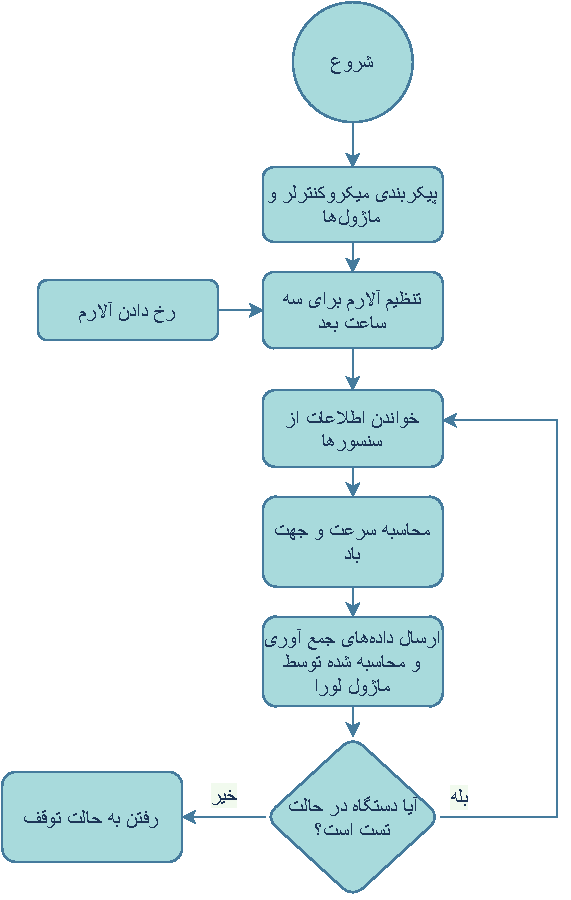
\includegraphics[width=0.6\linewidth]{Assets/SensorFlowChart.pdf}
	\caption{فلوچارت برنامه سمت سنسور.}
	\label{fig:SensorFlowChart}
\end{figure}

\زیرقسمت{نحوه خواندن دما و فشار از سنسور \متن‌لاتین{BMP180}}
در ابتدا لازم است ضرایب کالیبراسیون از سنسور \متن‌لاتین{BMP180} دریافت شود. روش ارتباط این ماژول با میکروکنترلر از طریق پروتکل \متن‌لاتین{I2C} است. جهت خواندن مقادیر ضرایب کالیبراسیون باید آدرس \متن‌لاتین{MSB} رجیستر متناظر با هر ضریب را با مود \متن‌لاتین{Read} به آدرس ماژول (\متن‌لاتین{0x77}) ارسال نماییم و ماژول در پاسخ 16 بیت داده را به ما بر می‌گرداند که مقدار ضریب کالیبراسیون مورد نظر است. آدرس رجیستر‌های ضرایب کالیبراسیون در تصویر شکل \رجوع{fig:bmp180Calibrationcoefficient} آمده است.
\begin{figure}[H]
	\centering
	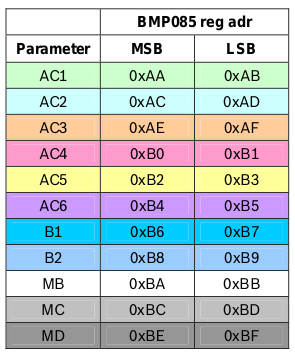
\includegraphics[width=0.5\linewidth]{Assets/bmp180Calibrationcoefficient.png}
	\caption{آدرس رجیستر ضرایب کالیبراسیون سنسور \متن‌لاتین{BMP180}.}
	\label{fig:bmp180Calibrationcoefficient}
\end{figure}

\زیرزیرقسمت{خواندن دما}
به جهت خواندن مقدار دما باید مقدار \متن‌لاتین{0x2E} را در رجیستر کنترل \متن‌لاتین{0xF4} بنویسیم. با این کار سنسور در حالت اندازه‌گیری دمای محیط قرار می‌گیرد و پس از حداکثر 4٫5 میلی ثانیه این داده برای خواندن آماده ‌می‌شود. این کار با ارسال مقدار آدرس رجیستر کنترل یعنی \متن‌لاتین{0xF4} در مود \متن‌لاتین{Write} به آدرس ماژول (\متن‌لاتین{0x77}) و پس از آن ارسال مقدار کنترل مورد نظر یعنی \متن‌لاتین{0x2E} انجام می‌شود. پس از اندازه‌گیری دما مقدار اندازه‌گیری شده در رجیستری با آدرس \متن‌لاتین{(MSB)0xF6} و \متن‌لاتین{(LSB)0xF7} در ماژول ذخیره می‌شود. به جهت خواندن مقدار اندازه‌گیری شده پس از حداقل 4٫۵ میلی ثانیه بعد از ارسال مقدار کنترلر \متن‌لاتین{0x2E} به ماژول باید مقدار \متن‌لاتین{MSB} رجیستر داده‌هایعنی \متن‌لاتین{0xF6} به آدرس سنسور (\متن‌لاتین{0x77}) در مود \متن‌لاتین{Read} فرستاده شود تا ماژول در پاسخ 16 بیت داده‌های اندازه گیری شده را که در این حالت مقدار دمای محیط است را به ما برگرداند (ابتدا مقدار رجیستر \متن‌لاتین{MSB} و سپس مقدار \متن‌لاتین{LSB} برگشت داده می‌شود). سپس مقدار دقیق دمای محیط با دقت 0.1 درجه سانتی گراد از طریق فرمول زیر قابل محاسبه خواهد بود:
\begin{fleqn}
	\begin{equation*}
		\begin{split}
			&UT = MSB << 8 + LSB \\
			&X1 = (UT - AC6) * AC5 / 2^{15} \\
			&X2 = MC * 2^{11} / (X1 + MD) \\
			&B5 = X1 + X2 \\
			&T = (B5 + 8) / 2^4
		\end{split}
	\end{equation*}
\end{fleqn}
\noindent
که $AC6$، $AC5$، $MD$ و $MC$ ضرایب کالیبراسیون، $MSB$ مقدار \متن‌لاتین{MSB} رجیستر داده‌های دریافت شده، $LSB$ مقدار \متن‌لاتین{LSB} رجیستر داده‌های دریافت شده و $T$ دمای محیط بر حسب سانتی‌گراد خواد بود.

\زیرزیرقسمت{خواندن فشار}
طریقه خواندن فشار از ماژول نیز مشابه خواندن دما است. در ابتدا لازم باید مقدار رجیستر کنترل ماژول را با مقدار مورد نظر (که در اینجا مقدار متناظر با دریافت فشار است) پر کرد و پس از زمانی مشخص داده‌های اندازه گیری شده را از رجیستر‌های داده ماژول خواند. در حالت خواندن فشار بر خلاف خواندن دما ماژول حالت‌های نمونه‌بردادی مختلفی را ارائه می‌کند که باید بر اساس نیاز مقدار مربوط به هر مود نمونه برداری که مد نظر بود را در رجیستری کنترل نوشت تا ماژول در حالت نمونه برداری مورد نظر قرار گیرد. با افزایش نرخ نمونه برداری دقت مقدار اندازه‌گیری شده بیشتر شده ولی زمانی که ماژول صرف اندازه‌گیری می‌کند نیز افزایش می‌یابد. در جدول \رجوع{table:BMP180persure} مقدار رجیستر کنترلی متناظر با هر مود نمونه برداری و حداکثر زمان لازم برای انجام نمونه برداری آورده شده است. 

\begin{table}[!h]
	\centering
	\caption{حالت‌های نمون برداری فشار ماژول \متن‌لاتین{BMP180}.}
	\label{table:BMP180persure}
	\begin{tabular}{ccc}
		حالت نمونه برداری & مقدار رجیستر کنترلی & حداکثر زمان اندازه‌گیری (میلی‌ثانیه)\\
		\hline
		0 & \متن‌لاتین{0x34} & 4٫5 \\
		1 & \متن‌لاتین{0x74} & 7٫5 \\
		2 & \متن‌لاتین{0xB4} & 13٫5 \\
		3 & \متن‌لاتین{0xF4} & 25٫5 \\
		
	\end{tabular}
\end{table}

در این پروژه استفاده از مود نمونه برداری 0 برای ما کفایت می‌کند. برای محاسبه فشار اندازه گیری دمای هوا نیز لازم است پس ابتدا لازم است قبل از درخواست اندازه گیری فشار دمای محیط توسط روشی که قبل تر گفته شد اندازه گیری شود. به جهت خواندن مقدار فشار باید مقدار \متن‌لاتین{0x34} را در رجیستر کنترل \متن‌لاتین{0xF4} بنویسیم (مود 0). با این کار سنسور در حالت اندازه‌گیری فشار قرار می‌گیرد و پس از حداکثر 4٫5 میلی ثانیه (با توجه به جدول \رجوع{table:BMP180persure} و در مود 0) این داده برای خواندن آماده ‌می‌شود. این کار با ارسال مقدار آدرس رجیستر کنترل یعنی \متن‌لاتین{0xF4} در مود \متن‌لاتین{Write} به آدرس ماژول (\متن‌لاتین{0x77}) و پس از آن ارسال مقدار کنترل مورد نظر یعنی \متن‌لاتین{0x34} انجام می‌شود. پس از اندازه‌گیری فشار مقدار اندازه‌گیری شده در رجیستری با آدرس \متن‌لاتین{(MSB)0xF6}،\متن‌لاتین{(LSB)0xF7} و \متن‌لاتین{0xF8(XLSB)} در ماژول ذخیره می‌شود. به جهت خواندن مقدار اندازه‌گیری شده پس از حداقل 4٫۵ میلی ثانیه بعد از ارسال مقدار کنترل \متن‌لاتین{0x34} (در مود 0) به ماژول باید مقدار \متن‌لاتین{MSB} رجیستر داده‌هایعنی \متن‌لاتین{0xF6} به آدرس سنسور (\متن‌لاتین{0x77}) در مود \متن‌لاتین{Read} فرستاده شود تا ماژول در پاسخ 16 بیت داده‌های اندازه گیری شده را به ما برگرداند (ابتدا مقدار رجیستر \متن‌لاتین{MSB} و سپس مقدار \متن‌لاتین{LSB} برگشت داده می‌شود) و سپس باید مقدار \متن‌لاتین{XLSB} رجیستر داده‌هایعنی \متن‌لاتین{0xF8} به آدرس سنسور (\متن‌لاتین{0x77}) در مود \متن‌لاتین{Read} فرستاده شود تا ماژول در پاسخ 8 بیت داده‌ را به ما برگرداند. سپس مقدار دقیق فشار محیط با دقت 1 پاسکال از طریق فرمول زیر قابل محاسبه خواهد بود:

\begin{fleqn}
	\begin{equation*}
	\begin{split}
		&UP = (MSB<<16 + LSB<<8 + XLSB) >> (8-oss) \\
		&B6 = B5 - 4000 \\
		&X1 = (B2 * (B6 * B6 / 2^{12} )) / 2^{11}\\
		&X2 = AC2 * B6 / 2^{11}\\
		&X3 = X1 + X2\\
		&B3 = ((AC1*4+X3) << oss + 2) / 4\\
		&X1 = AC3 * B6 / 2^{13}\\
		&X2 = (B1 * (B6 * B6 / 2^{12} )) / 2^{16}\\
		&X3 = ((X1 + X2) + 2) / 2^2\\
		&B4 = AC4 * (unsigend long)(X3 + 32768) / 2^{15}\\
		&B7 = ((unsigned long)UP - B3) * (50000 >> oss)\\
		&if (B7 < 0x80000000) \{ p = (B7 * 2) / B4 \}\\
	\end{split}
	\end{equation*}
\end{fleqn}

\begin{fleqn}
	\begin{equation*}
	\begin{split}
		&else \{ p = (B7 / B4) * 2 \}\\
		&X1 = (p / 2^8 ) * (p / 2^8 )\\
		&X1 = (X1 * 3038) / 2^{16}\\
		&X2 = (-7357 * p) / 2^{16}\\
		&p = p + (X1 + X2 + 3791) / 2^{16}
		\end{split}
	\end{equation*}
\end{fleqn}
\noindent
که $B5$ مقدار بدست آمده از روابط محاسبه دما است که در بخش قبلی بیان شده است، $oss$ عدد مود نرخ نمونه برداری (از 0 تا 3 مطابق جدول \رجوع{table:BMP180persure})، $AC1$، $AC2$، $AC3$، $AC4$، $B1$ و $B2$ ضرابیب کالیبراسیون، $MSB$ مقدار \متن‌لاتین{MSB} رجیستر داده‌های دریافت شده، $LSB$ مقدار \متن‌لاتین{LSB} رجیستر داده‌های دریافت شده ، $XLSB$ مقدار رجیستر داده \متن‌لاتین{XLSB} و در نهایت p مقدار فشار اندازه‌گیری شده بر حسب پاسکال خواهد بود. 

\زیرقسمت{نحوه خواندن شدت نور از سنسور \متن‌لاتین{MAX44009}}
در ابتدا پس از روشن شدن ماژول لازم است که حالت کاری ماژول و تنظیمات اولیه آن انجام شود. این کار با نوشتن رجیستر کنترلی این ماژول با آدرس \متن‌لاتین{0x02} انجام می‌شود. بیت هشتم این رجیستر به بین \متن‌لاتین{CONT} معروف است. این بیت مسئول تعیین مود کارکرد است به طوری که اگر مقدار $0$‍ در آن نوشته شود ماژول هر 800 میلی‌ثانیه مقدار نور محیط را اندازه‌گیری کرده و در رجیتسر‌های خود ذخیره می‌کند و اگر مقدار $1$ در آن نوشته شده باشد ماژول بدون وقفه و پشت‌سر‌هم اندازه‌گیری نور را انجام می‌دهد. برای این پروژه استفاده از مود $0$ مناسب تر است و ازین مود استفاده خواهیم کرد. بیت هفتم این رجیستر به بیت \متن‌لاتین{MANUAL} معروف است و در صورتی که با $1$ پر شود کاربر قادر به مشخص کردن مقادیر \متن‌لاتین{CDR} و \متن‌لاتین{TIM[2:0]} خواهد بود و در غیر این صورت خوده سیستم در مورد این مقادیر تصمیم گیری می‌کند. مقدار \متن‌لاتین{CDR} که بیت چهارم رجیستر کنترل است، مشخص کننده مقدار مقسم مقادیر خوانده شده از \متن‌لاتین{ADC} است و در صورتی که با $0$ پر شده باشد هیچ عملیات تقسیمی رخ نداده و مقادیر \متن‌لاتین{ADC} عینا در رجیستر‌ها کپی می‌شوند و در صورتی که با مقدار $1$ پر شده باشد مقادیر تقسیم بر 8 می‌شوند (در مواقعی که نور محیط بسیار زیاد است کاربرد دارد). مقدار \متن‌لاتین{TIM[2:0]} نیز که بیت اول تا سوم رجیستر کنترل را به خود اختصاص داده بیان کننده زمان نمونه برداری و اذغام است که مقادیر متناظر با حالت‌های مختلف قابل انتخاب برای این بیت‌ها در جدول \رجوع{table:BMP180persure} آمده است. در حالت خودکار زمان‌هایی بین 100 تا 800 میلی ثانیه انتخاب می‌شوند و در حالت دستی میتوان از 6.25 میلی ثانیه تا 800 میلی ثانیه را انتخاب کرد. حالت 800 میلی ثانیه مناسب محیط با نور بسیارکم و حالت 6.25 میلی ثانیه مناسب محیط‌هایی با نور بسیار زیاد است. 

\begin{table}[!h]
	\centering
	\caption{مقادیر بیت‌های \متن‌لاتین{TIM[2:0]}.}
	\label{table:BMP180persure}
	\begin{tabular}{c|c}
		\متن‌لاتین{TIM[2:0]} & زمان نمونه برداری و ادغام (میلی‌ثانیه)\\
		\hline
		$000$ & 800 \\
		$001$ & 400 \\
		$010$ & 200 \\
		$011$ & 100 \\
		$100$ & 50 \\
		$101$ & 25 \\
		$110$ & 12٫5 \\
		$111$ & 6٫25 \\
	\end{tabular}
\end{table}
\noindent
در این پروژه به دلیل ثابت نبودن شرایط محیطی انتخاب حالت خودکار (مقدار $0$ برای \متن‌لاتین{MANUAL}) مناسب ترین روش ممکن است. با این کار مقادیر \متن‌لاتین{CDR} و \متن‌لاتین{TIM[2:0]} توسط خوده ماژول و با توجه به شرایط محیطی در هر اندازه گیری مشخص می‌شود. پس در این پروژه لازم است پس از روشن شدن ماژول مقدار \متن‌لاتین{0x00} در رجیستر کنترل به آدرس \متن‌لاتین{0x02} نوشته شود. این کار با ارسال آدرس رجیستر (\متن‌لاتین{0x02}) در مود \متن‌لاتین{Write} به آدرس ماژول (\متن‌لاتین{0x4A}) و پس از آن ارسال مقدار \متن‌لاتین{0x00} انجام می‌شود. با این کار ماژول ماکسیموم هر 800 میلی ثانیه یک بار دیتا‌های جدید را اندازه‌گیری کرده و در رجیستر‌هایی با آدرس \متن‌لاتین{0x03(MSB)} و \متن‌لاتین{0x04(LSB)} ذخیره می‌کند به جهت خواندن این مقادیر لازم است آدرس رجیستر به آدرس ماژول در مود \متن‌لاتین{Read} فرستاده شود تا ماژول در پاسخ 8 بیت دیتای این رجیستر‌ها را به ما برگرداند. پس از دریافت این مقادیر شدت نور بر حسب لوکس از طریق روابط زیر قابل محاسبه خواهد بود:
\begin{fleqn}
	\begin{equation*}
		Lux = (2^{Exponent} \times Mantissa) \times 0.045
	\end{equation*}
\end{fleqn}
\noindent
که مقادیر $Exponent$ و $Mantissa$ از روی مقادیر رجیستر‌های \متن‌لاتین{0x03(MSB)} و \متن‌لاتین{0x04(LSB)} و از طریق روابط زیر و جدول \رجوع{table:MAX44009DataRegisters} بدست می‌آیند.

\begin{table}[!h]
	\centering
	\caption{مقدار رجیستر‌های \متن‌لاتین{0x03(MSB)} و \متن‌لاتین{0x04(LSB)}.}
	\label{table:MAX44009DataRegisters}
	\begin{tabular}{c|cccccccc}
		رجیستر & $bit 0$ & $bit 1$ & $bit 2$ & $bit 3$ & $bit 4$ & $bit 5$ & $bit 6$ & $bit 7$\\
		\hline
		\متن‌لاتین{0x03} & $M4$ & $M5$ & $M6$ & $M7$ & $E0$ & $E1$ & $E2$ & $E3$ \\
		\متن‌لاتین{0x04} & $M0$ & $M1$ & $M2$ & $M3$ & - & - & - & - \\
	\end{tabular}
\end{table}


\begin{fleqn}
	\begin{equation*}
		Exponent = 8\times E3 + 4\times E2 + 2\times E1 + E0\\
	\end{equation*}
\end{fleqn}
\begin{fleqn}
	\begin{equation*}
	\begin{split}
		Mantissa = &128\times M7 + 64\times M6 + 32\times M5 + 16\times M4 \\
					&+ 8\times M3 + 4\times M2 + 2\times M1 + M0
	\end{split}
	\end{equation*}
\end{fleqn}


\زیرقسمت{نحوه دریافت جهت جغرافیایی از سنسور \متن‌لاتین{QMC5883L}}
در ابتدا پس از روشن شدن ماژول لازم است رجیستر‌ کانفیک این ماژول تنظیم شده و ماژول در مود کاری مورد نظر قرار بگیرد. بیت‌ها و تنظیمات متناظر با اطلاعات پر شده در این رجیستر در جدول تصویر \رجوع{fig:QMC5883LControlRegister} قابل مشاهده است. 

\begin{figure}[H]
	\centering
	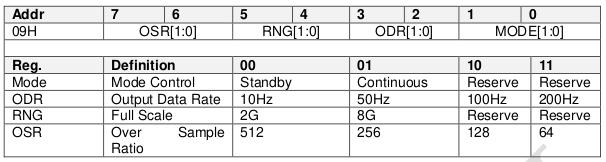
\includegraphics[width=0.9\linewidth]{Assets/QMC5883LControlRegister.png}
	\caption{رجیستر کانفیگ ماژول \متن‌لاتین{QMC5883L}.}
	\label{fig:QMC5883LControlRegister}
\end{figure}
\noindent
برای شروع به کار و نمونه برداری، مود کاری باید در حالت \متن‌لاتین{continuous} قرار بگیرد.  برای این پروژه ریت خروجی 10 یا 50 هرتز و ریت نمونه برداری 2 گاوس مناسب اند. مقدار \متن‌لاتین{OSR} را نیز بیشترین حالت یعنی 512 در نظر می‌گیریم. پس مقدار رجسیتر کانفیگ باید با \متن‌لاتین{0x05} پر شود. برای این کار باید مقدار آدرس رجیستر کانفیگ (\متن‌لاتین{0x09}) را به در مود \متن‌لاتین{Write} به آدرس ماژول (\متن‌لاتین{0x0D}) ارسال کنیم و پس از آن مقدار مورد نظر را (\متن‌لاتین{0x05}) ارسال نماییم. با این کار ماژول وارد مود کار بدون وقفه خود شده و پس از اندازه گیری‌ و ذخیره اطلاعات در رجیستر‌های خود اولین بیت رجیستر حالت خود به آدرس \متن‌لاتین{0x06} را به نشانه وجود داده برای دریافت 1 می‌کند. پس با خواندن رجیستر حالت این ماژول میتوانیم از وجود یا عدم وجود داده برای دریافت باخبر شویم. این کار را با ارسال آدرس رجیستر حالت (\متن‌لاتین{0x06}) در مود \متن‌لاتین{Read} به آدرس ماژول (\متن‌لاتین{0x0D}) انجام می‌دهیم و ماژول در پاسخ 8 بیت داده‌های رجیستر حالت را به ما برمی‌گرداند. در صورت 1 بودن اولین بیت رجیستر حالت داده‌ها برای دریافت آماده‌اند و لازم است آن‌ها را از رجیستر‌های داده بخوانیم. رجیستر‌های \متن‌لاتین{0x00(LSB)} و \متن‌لاتین{0x01(MSB)} حاوی اطلاعات محور \متن‌لاتین{X}، رجیستر‌های \متن‌لاتین{0x02(LSB)} و \متن‌لاتین{0x03(MSB)} حاوی اطلاعات محور \متن‌لاتین{Y} و رجیستر‌های \متن‌لاتین{0x05(LSB)} و \متن‌لاتین{0x06(MSB)} حاوی اطلاعات محور \متن‌لاتین{Z} هستند. با دریافت این اطلاعات به راحتی با انجام محاسبات ریاضی میتوان زاویا با محور‌های مختصات را بدست آورد. در این پروژه زاویه بردار روی صفحه \متن‌لاتین{X} و متن‌لاتین{Y} با بردار \متن‌لاتین{X} برای ما اهمیت دارد که با توجه به فرمول زیر بدست می‌آید:

\begin{fleqn}
	\begin{equation*}
		angle = \arctan{\frac{Y}{X}}
	\end{equation*}
\end{fleqn}

\زیرقسمت{نحوه خواندن رطوبت از سنسور \متن‌لاتین{AHT10}}
این سنسور بر خلاف سنسور‌های دیگه نیازی به کانفیگ برای اندازه‌گیری و کالیبراسیون ندارد و پس از روشن شدن میتوان آن را در حالت دریافت اطلاعات قرار داد و پس از حداقل 75 میلی‌ثانیه داده‌ها را از این سنسور خواند. این سنسور علاوه بر رطوبت دمای هوا را نیز اندازه گیری می‌کند ولی دقت آن در اندازه‌گیری دمای هوا به اندازه ماژول \متن‌لاتین{BMP180} نیست و از این رو داده‌های دمای هوایی که این سنسور اندازه‌گیری می‌کند را در این پروژه نادیده می‌گیریم.

برای قرار گرفتن ماژول در مود اندازه‌گیری باید دیتا‌های \متن‌لاتین{0xAC}، \متن‌لاتین{0x33} و \متن‌لاتین{0x00} را به همین ترتیب به آدرس ماژول (\متن‌لاتین{0x38}) ارسال کرد. با این کار ماژول ر حالت اندازه‌گیری قرار میگیرد و حداقل 75 میلی‌ثانیه بعد دیتا‌های اندازه‌گیری شده را در قالب 48 بیت به ما برمی‌گرداند این دیتا‌ها را هر هشت بیت با نام \متن‌لاتین{Data0} تا \متن‌لاتین{Data5} نام گذاری می‌کنیم. فشار نسبی هوا برحسب درصد از طریق روابط زیر و با استفاده از مقادیر برگشت داده شده از ماژول قابل محاسبه خواهد بود:

\begin{fleqn}
	\begin{equation*}
	\begin{split}
		&S_{RH} = Data1 \times 2^{12} +  Data2 \times 2^4 + Data3 / 2^4\\
		&RH = (S_{RH} * 100 / 2^{20});
	\end{split}
	\end{equation*}
\end{fleqn}

که $Data1$ تا $Data3$ مقادیر برگشت داده شده از سنسور و $RH$ مقدار رطوبت نسبی برحسب درصد است. 

\زیرقسمت{نحوه محاسبه سرعت و جهت باد}
جهت محاسبه سرعت و جهت باد ابتدا باید سرعت باد روی دو محور \متن‌لاتین{X} و \متن‌لاتین{Y} را بدست آورد. برای این کار در ابتدا نیاز به محاسبه سرعت صوت خواهد بود. سرعت صوت با توجه به روابطی که در بخش \رجوع{sec:windSpeedANDAngle} بیان شده است به عنوان تابعی از دمای هوا، رطوبت و فشار قابل محاسبه است. با وجود فاصله‌ای ثابت و مشخص بین فرستنده و گیرنده‌های آلتراسونیک،بنا به روابط بیان شده در بخش \رجوع{sec:windSpeedANDAngle}، زمانی که طول می‌کشد موج آلتراسونیک از فرستنده به گیرنده برسد با سرعت صورت به اضافه سرعت باد متناسب خواهد بود. پس با داشتن سرعت صوت و فاصله بین گیرنده و فرستنده و محاسبه زمانی که طول می‌کشد موج آلتراسونیک از فرستنده به گیرنده برسد می‌توان سرعت باد را محاسبه کرد.

برای محاسبه زمانی که طول می‌کشد تا موج آلتراسونیک از فرستنده به گیرنده برسد از ماژول \متن‌لاتین{HCSR05} بهره گرفتیم. این ماژول با دریافت پالسی با طول حداقل 10 میکرو ثانیه، موج آلتراسونیکی با فرکانس 40 کیلوهرتز تولید می‌کند. این ماژول هنگامی که پالس آلتراسونیک را تولید و ارسال می‌کند خروجی خود را 1 می‌کند و آن را تا زمانی که پالس آلتراسونیک را از گیرنده خود دریافت کند 1 نگه‌می‌دارد. در حقیقت با اندازه‌گیری طول پالس تولید شده در خروجی این ماژول زمانی که طول می‌کشد پالس آلتراسونیک از گیرنده به فرستنده برسد بدست می‌آید (این زمان به زمان پرواز معروف  است). این زمان را با استفاده از واحد تایمر در میکروکنترلر اندازه‌گیری میکنیم به طوری که زمانی که پالسی با لبه بالا رونده روی پایه خروجی ماژول رخ داد شمارش تایمر را شروع کرده و هر یک میکرو ثانیه (دقت خروجی ماژول در این حد است) شمارش می‌کند و سپس زمانی که پالسی با لبه پایین رونده رخ داد شمارش را متوقف می‌کند و عدد شمارنده در این حالت همان زمان به اصطلاح پرواز ما خواهد بود.

با محاسبه زمان پرواز و با توجه به روابط ارائه شده در بخش \رجوع{sec:windSpeedANDAngle} میتوان سرعت باد را بدست آورد. برای محاسبه جهت باد لازم است سرعت باد روی هر دو محور مختصاتی \متن‌لاتین{X} و \متن‌لاتین{Y} بدست بیاید. با داشتن سرعت باد روی هر دو محور میتوان این مقادیر را به دستگاه مختصات قطبی برد تا اندازه و زاویه وزش باد نسبت به محور \متن‌لاتین{X} مختصات را در دست داشت. در این حالت اندازه در مختصات قطبی همان سرعت باد مد نظر ما است و با جمع کردن زاویه بدست آمده در این حالت با زاویه بدست آمده از سنسور قطب نما ($angle$) جهت باد بدست می‌آید. البته لازم است در این حالت محور‌های مختصات سنسور باد منطبق با محور‌های مختصات سنسور قطب‌نما باشند در غیر این صورت باید اختلاف زاویه این دو محور مختصات را نیز در محاسبات لحاظ کرد.

\زیرقسمت{نحوه ارسال اطلاعات از طریق لورا}\label{sec:loraConfig}
در ابتدا پس از روشن کردن لورا باید مقادیر رجیستر‌های کانفیگ آن را با مقادیر مورد نیاز پر کرد و آن را در مود کاری مورد نیاز قرار داد. به جهت نوشتن رجیستر‌های کانفیگ لورا باید در ابتدا این ماژول را در مود اسلیپ قرار داد. تنها در این حالت مقادیر نوشته شده به عنوان کانفیگ روی ماژول اعمال می‌شوند. برای این کار باید مقدار رجیستر \متن‌لاتین{RegOpMode} با آدرس \متن‌لاتین{0x01} با مقدار \متن‌لاتین{0x08} پر شود. برای این کار پس از انتخاب چیپ با پایه \متن‌لاتین{NSS}، مقدار \متن‌لاتین{0x01} و سپس \متن‌لاتین{0x08} روی پایه \متن‌لاتین{MOSI} ارسال می‌شود. با این کار ماٰژول لورا در حالت اسپیلپ و آماده اعمال تنظیمات قرار می‌گیرد. حال مقدار رجیستر‌های \متن‌لاتین{RegFrMsb}، \متن‌لاتین{RegFrMid} و \متن‌لاتین{RegFrLsb} به آدرس‌های \متن‌لاتین{0x06}، \متن‌لاتین{0x07} و \متن‌لاتین{0x08} را که تنظیم کننده فرکانس موج رادیویی اند را با مقادیر \متن‌لاتین{0x6C}، \متن‌لاتین{0x40} و \متن‌لاتین{0x00} پر میکنیم (این مقدار از تقسیم فرکانس مورد نظر بر  61٫03515625 بدست آمده است). با این کار فرکانس کاری روی 433 مگاهرتز تنظیم می‌شود. حال باید رجیستر \متن‌لاتین{RegPaConfig} به آدرس \متن‌لاتین{0x09} را مقدار دهی کنیم. این رجیستر تنظیم کننده توان خروجی است. برای توان خروجی 20 \متن‌لاتین{dB} باید مقدار \متن‌لاتین{0x8F} را در این رجیستر قرار دهیم. برای قرار دادن پهنای باند ماژول در حالت 250 کیلو هرتز لازم است 4 بیت آخر رجیستر \متن‌لاتین{RegModemConfig1} به آدرس \متن‌لاتین{0x1D} با مقدار \متن‌لاتین{0b1000} پر شود. همچنین برای تعیین ضریب پخش 10 لازم است 4 بیت آخر رجیستر رجیستر \متن‌لاتین{RegModemConfig2} به آدرس \متن‌لاتین{0x1E} با مقدار \متن‌لاتین{0b1010} پر شود. به جهت دریافت وضعیت ارسال پیام از طریق پایه‌های \متن‌لاتین{DIO} لازم است بیت اول رجیستر \متن‌لاتین{RegDioMapping2} با مقدار \متن‌لاتین{1} پر شود. در این حالت در صورت ارسال داده‌ها پایه \متن‌لاتین{DIO0} فعال می‌شود و ما با چک کردن وضعیت این پایه بعد از اعمال دستور ارسال می‌توانیم از وضعیت ارسال بسته باخبر شویم. 

\begin{figure}[H]
	\centering
	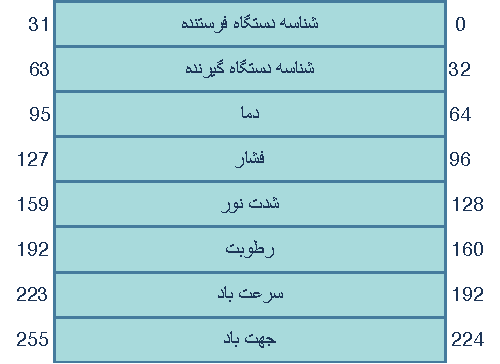
\includegraphics[width=0.6\linewidth]{Assets/sensorData.pdf}
	\caption{ساختار داده‌های موجود در سمت سنسور.}
	\label{fig:sensorData}
\end{figure}

پس از تنظیم رجیستر‌های کانفیگ ماژول را به حالت اسندبای میبریم در این حالت دیگر رجیستر‌های کانفیگ قابل تغییر نخواهند بود. برای این کار مقدار \متن‌لاتین{0x09} را درون رجیستر \متن‌لاتین{RegOpMode} می‌نویسیم. جهت ارسال داده باید رجیستر \متن‌لاتین{RegFifo} را با داده‌ مورد نظر پر کرد و سپس مود کاری را در حالت \متن‌لاتین{Tx} قرار‌ داد. برای قرار دادن ماژول در مود \متن‌لاتین{Tx} تنها کافیست مقدار \متن‌لاتین{0x8B} را درون رجیستر \متن‌لاتین{RegOpMode} (با آدرس \متن‌لاتین{0x01}) نوشت. داده‌های دریافت شده در سمت سنسور در آرایه‌ای از نوع \متن‌لاتین{float} ذخیره شده اند. ساختار این داده‌ها را در تصویر \متن‌لاتین{fig:sensorData} مشاهده می‌کنید. برای جای دادن داده‌ها در رجیستر \متن‌لاتین{FIFO} ماژول لورا لازم است داده‌ها در ساختاری 8 بیتی (آرایه‌ای از اعداد بدون علامت 8 بیتی) برای ماژول ارسال شوند از این رو مقادیر موجود در آرایه داده‌ها هر 8 بیت به هشت بیت به ماژول لورا و رجیستر \متن‌لاتین{FIFO} این ماژول فرستاده می‌شوند. ساختار داده‌های ارسالی به رجیستر \متن‌لاتین{FIFO} لورا نیز در تصویر \رجوع{fig:loraData} قابل مشاهده است. این داده‌ها با همین ساختار به طرف ایستگاه فرستاده و دریافت می‌شوند و لازم است پس از دریافت دوباره به ساختار اصلی و قبلی خود تبدیل شوند. 

\begin{figure}[H]
	\centering
	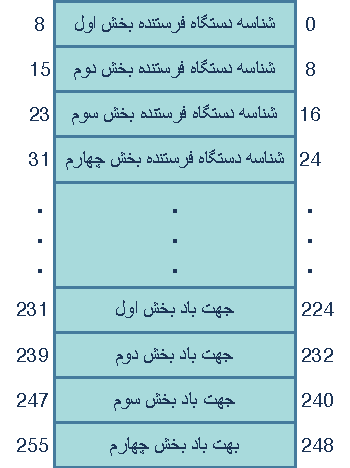
\includegraphics[width=0.4\linewidth]{Assets/loraData.pdf}
	\caption{ساختار داده‌های ارسالی از طریق لورا.}
	\label{fig:loraData}
\end{figure}

\زیرقسمت{پیکربندی \متن‌لاتین{I2C}}
برای نوشتن کد‌های این پروژه از لایبری \متن‌لاتین{HAL} استفاده می‌کنیم. در این صورت برای فعال کردن بخش \متن‌لاتین{I2C} تنها لازم است این بخش را در نرم افزار \متن‌لاتین{STM32CubeMX} فعال کنیم. تنظیمات این بخش مثل سرعت و نوع آدرس وابسته به دستگاه‌های \متن‌لاتین{Slave} متصل به \متن‌لاتین{I2C} است و باید با توجه به مواردی که آن‌ها پشتیبانی می‌کنند تنظیمات این قسمت را پر کرد. خوشبختانه تمامی سنسور‌های استفاده شده برای این پروژه تنظیمات یکسانی را پشتیبانی می‌کنند و می‌توان تنها با یک \متن‌لاتین{I2C} با تمامی آن‌ها ارتباط برقرار و دیتا‌های لازم را دریافت کرد. سنسور‌های استفاده شده همگی از ماکسیموم سرعت قابل استفاده یعنی 400 کیلوهرتز پشتیبانی می‌کنند اما در مورد این پروژه سرعت تبادل داده‌ها با سنسور‌ها تفاوت زیادی نمی‌کند. پس در نتیجه سرعت 100 کیلوهرتز را برای تست وتوسعه به امید کمتر کردن خطا‌های ممکن انتخاب می‌کنیم. تصویر تنظیمات این بخش در نرم افزار \متن‌لاتین{STM32CubeMX} در شکل \رجوع{fig:i2cConfig} آمده است. 

\begin{figure}[H]
	\centering
	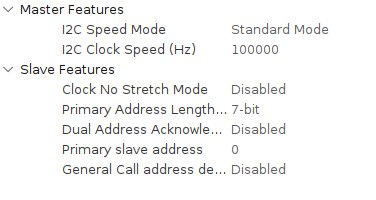
\includegraphics[width=0.6\linewidth]{Assets/i2cConfig.png}
	\caption{تنظیمات \متن‌لاتین{I2C}.}
	\label{fig:i2cConfig}
\end{figure}

\زیرقسمت{پیکربندی \متن‌لاتین{SPI}}
به سبب اسفاده از لایبری \متن‌لاتین{HAL} و نرم افزار \متن‌لاتین{STM32CubeMX} برای فعال کردن این بخش از میکروکنترلر تنها کافی است این بخش را در نرم اقزار \متن‌لاتین{STM32CubeMX} فعال کنیم. برای این کار \متن‌لاتین{SPI} مورد نظر را در حالت \متن‌لاتین{Full-Duplex Master} قرار می‌دهیم. تنظیم پارامتر‌های دیگر بستگی به تنظیمات قابل پشتیبانی برای \متن‌لاتین{Slave}‌ها دارد. در این حالت برای ماژول لورا تنظیمات تصویر \رجوع{fig:SPIConfig} را اعمال می‌کنیم. ماژول لورا سرعت‌های تبادل بالاتر را نیز ساپورت می‌کند ولی در این پروژه سرعت تبادلات تفاوت زیادی ایجاد نمی‌کند از این رو برای تست وتوسعه به استفاده از سرعت‌های تبادل پایین تر بسنده می‌کتیم. 

\begin{figure}[H]
	\centering
	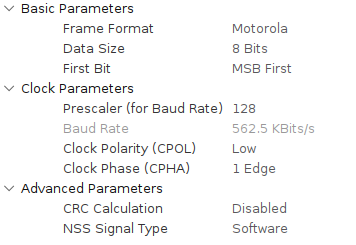
\includegraphics[width=0.6\linewidth]{Assets/SPIConfig.png}
	\caption{تنظیمات \متن‌لاتین{SPI}.}
	\label{fig:SPIConfig}
\end{figure}
\زیرقسمت{حالت توقف میکروکنترلر}
در این پروژه لازم است اطلاعات سنسور‌ها هر 3 ساعت یکبار جمع آوری و از طریق ماژول لورا مخابره شود و در بین این ساعات میکرو عملکرد دیگری نخواد داشت. برای ذخیره انرژی میتوان میکرو را در بین این ساعات در حالت توقف یا \متن‌لاتین{Stop} قرار داد. در حالت توقف مصرف انرژی میکرو کنترلر با غیر فعال کردن کلاک‌ها بسیار کاهش می‌یابد. در این مود مقادیر رم و رجیستر‌ها حفظ می‌شود و فقط کلاک‌ها غیر فعال می‌شوند. بعد از برخواستن از این حالت سیستم از کلاک \متن‌لاتین{HSI} به عنوان منبع کلاک استفاده می‌کند که لازم است در این حالت برای برگشت به حالت کار عادی تنظیمات کلاک دوباره اعمال شوند. در این حالت میکروکنترلر تنها مصرفی در حدود 0٫8 میکروآمپر را دارا می‌باشد (با فعال بودن \متن‌لاتین{RTC}). 

تفاوت این حالت با حالت \متن‌لاتین{Standby} که در آن میکرو کمترین میزان مصرف انرژی خود را دارد در این است که در حالت \متن‌لاتین{Standby} مقادیر رجیستر‌ها و رم ذخیره نمی‌شود (فقط رجیستر‌های مربوط به حالت \متن‌لاتین{Standby} دست نخورده باقی می‌مانند و باقی اطلاعات از دست می‌روند) و میکرو پس از برخواستن از این حالت وضعیتی مشابه وضعیت ریست شدن را خواهد داشت اما می‌توان مصرف را در حالتی مشابه تا 0٫57 میکرو‌آمپر کاهش داد.

برای خارج کردن میکروکنترلر از این حالت می‌توان از اینتراپت خارجی و یا آلارم واحد \متن‌لاتین{RTC} استفاده کرد. در این پروژه ما از آلارم واحد \متن‌لاتین{RTC} استفاده می‌کنیم. اولین آلارم را میتوان با استفاده از نرم افزار \متن‌لاتین{STM32CubeMX} در بخش \متن‌لاتین{RTC} تنظیم کرد و پس از آن با رخ دادن هر آلارم باید آلارم بعدی را برای سه ساعت بعد تنظیم کرد. 


\قسمت{ایستگاه}
فلوچارت فرآیند‌های سمت ایستگاه در تصویر \رجوع{fig:StationFlowChart} قابل مشاهده است شرح آن به قرار زیر است:
\شروع{فقرات}
\فقره 
با اتصال دستگاه از طریق کابل \متن‌لاتین{USB} به رایانه میکروکنترلر پس از فعال‌سازی بخش‌های موردنیاز، از طریق \متن‌لاتین{SPI} با ماژول لورا ارتباط برقرار کرده و رجیسترهای تنظیمات را با اطلاعات مشابه با سمت سنسور پر می‌کند و ماٰژول لورا را در حالت دریافت اطلاعات بدون توقف \پانویس{Continuously} قرارمی‌هد \مرجع{SX1278}.
\فقره 
میکرو به حلقه اصلی کار خود واردشده و پس از چک کردن وجود دیتای دریافتی در ماژول لورا، در صورت عدم وجود دیتا به حالت خواب \پانویس{Sleep} رفته و تا زمان دریافت دیتا در همان حالت باقی می‌ماند.
\فقره 
با دریافت دیتا توسط ماژول لورا وقفه‌ای خارجی رخ‌داده و میکرو را از حالت خواب بیدار می‌کند.
\فقره
میکرو کنترلر با برقراری ارتباط از طریق \متن‌لاتین{SPI} با ماژول لورا دیتای دریافت شده را خوانده و پس از بررسی یکسان بودن شناسه دریافت‌کننده با شناسه خود آن را از طریق \متن‌لاتین{USB} به رایانه ارسال می‌کند.
\فقره 
در صورت عدم وجود دیتاهای دیگر، میکرو کنترلر به حالت خواب رفته و تا رخ دادن وقفه بعدی، که نشان‌دهنده دریافت اطلاعات توسط ماژول لورا است، در همان حال باقی می‌ماند.
\پایان{فقرات}

\begin{figure}[H]
	\centering
	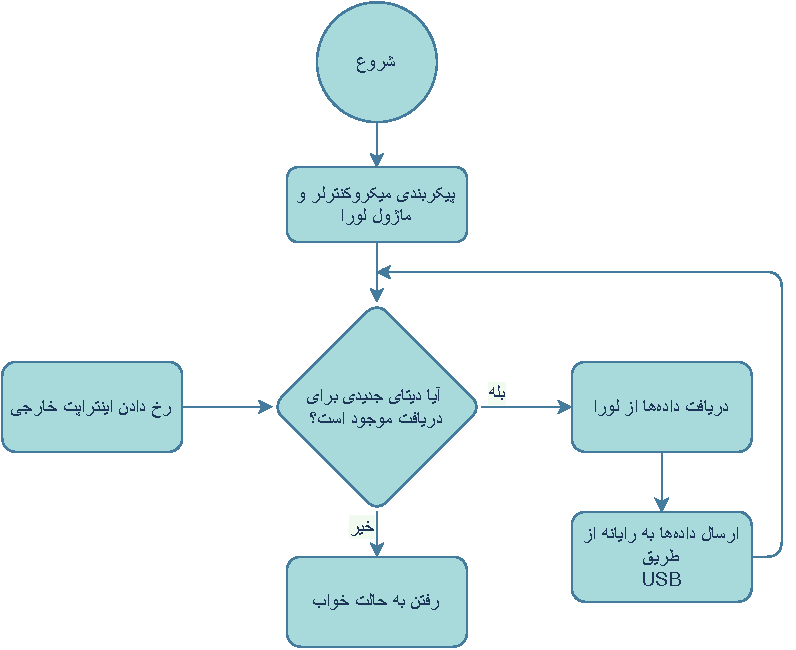
\includegraphics[width=0.7\linewidth]{Assets/StationFlowChart.pdf}
	\caption{فلوچارت برنامه سمت ایستگاه.}
	\label{fig:StationFlowChart}
\end{figure}

\زیرقسمت{نحوه دریافت اطلاعات از لورا}
برای اینکه ماژول لورا بتواند در این سمت اطلاعات ارسال شده را دریافت کند باید دقیقا همان تنظیماتی که در سمت سنسور برای آن اعمال شده در این سمت نیز اعمال شود. با وجود کوچک ترین تفاوتی بین پارامتر‌های فرکانس، پهنای‌باند و ضریب‌پخش بین دو سمت فرستنده و گیرنده دیگر ماژول لورا قادر نخواهد بود اطلاعات ارسال شده را دریافت کند. پس تمامی این پارامتر‌ها دقیقا مطابق بخش \رجوع{sec:loraConfig} در ماژول تنظیم خواهند شد. همچنین پیکربندی \متن‌لاتین{SPI} همانند پیکربندی بخش سنسور تنظیم شده است. 

پس از تنظیم این پارامتر‌ها ماژول لورا در این سمت باید در مود دریافت اطلاعات بدون توقف قرار داده شود. در این حالت در صورت دریافت اطلاعات ماژول روی پایه‌های \متن‌لاتین{DIO} خود با فعال کردن یکی از پایه‌ها (که قابل تنظیم است کذام پایه فعال شود) رخ دادن دریافت اطلاعات را اطلاع می‌دهد. در این حالت ماژول از کار باز نمی‌ایستد و دوباره منتظر دریافت اطلاعات می‌ماند. برای قرار دادن ماژول در این مود باید رجیستر \متن‌لاتین{RegOpMode} به آدرس \متن لاتین{0x01} با مقدار \متن‌لاتین{0x8D} پر شود. 

در این صورت در صورت رخ دادن دریافت داده میکرو‌کنترلر از طریق اینتراپت خارجی‌ای که به پایه \متن‌لاتین{DIO} ماژول وصل شده است از رخ دادن دریافت اطلاعات باخبر شده و می‌تواند جهت خواندن اطلاعات دریافت شده اقدام نماید. برای خواندن اطلاعات دریافت شده در ابتدا باید طول اطلاعات دریافت شده را از رجیستری با عنوان \متن‌لاتین{RegRxNbBytes} با آدرس \متن‌لاتین{0x13} دریافت کرد (ماکسیموم طول بسته قابل دریافت 256 بسته است). پس از آن با داشتن طول بسته می‌توان دیتای دریافت شده را از رجیستر‌های \متن‌لاتین{FIFO} (با آدرس \متن‌لاتین{0x00}) خواند. پس از خواندن اطلاعات موجود لازم است فلگ مربوط به اینتراپ را در ماژول ریست کرد برای این کار کافیست مقدار \متن‌لاتین{0xFF} را درون رجیستر \متن‌لاتین{RegIrqFlags} به آدرس \متن‌لاتین{0x12} نوشت. 

\begin{figure}[H]
	\centering
	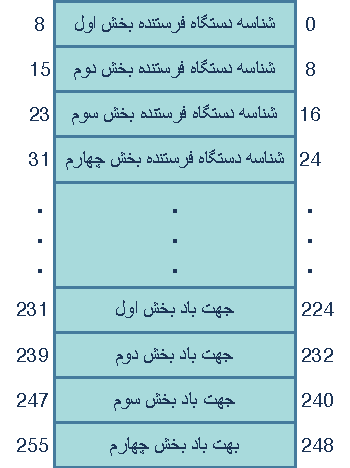
\includegraphics[width=0.4\linewidth]{Assets/loraData.pdf}
	\caption{ساختار داده‌های دریافت شده از طریق لورا.}
	\label{fig:loraDataReceive}
\end{figure}

داده‌های دریافت شده در این قسمت ساختاری مشابه ساختار داده‌های ارسال شده دارند (در تصویر \رجوع{fig:loraDataReceive} قابل مشاهده است). در این قسمت لازم است قبل از ارسال اطلاعات به رایانه شناسه دریافت کننده با شناسه موجود در دستگاه سمت ایستگاه چک شود. این کار برای جلو گیری از ثبت چند باره اطلاعات و یا جلو گیری از ثبت اطلاعات نادرست برای دستگاه‌هایی که همپوشانی رادیویی منطقه‌ای دارند لازم است. برای این کار باید ابتدا ساختار داده‌های دریافت شده که شامل 8x32 داده از نوع عدد بدون علامت می‌شود به ساختار اصلی که 32x8 داده‌ای و از نوع \متن‌لاتین{float} بوده است تبدیل شود این کار به سادگی و با تبدیل هر 4 جایگاه آرایه دیتا‌های دریافت شده به نوع \متن‌لاتین{float} انجام می‌شود. تصویر داده‌ها پس از تبدیل به ساختار اصلی در شکل \رجوع{fig:sensorDataConverted} آمده است.

\begin{figure}[H]
	\centering
	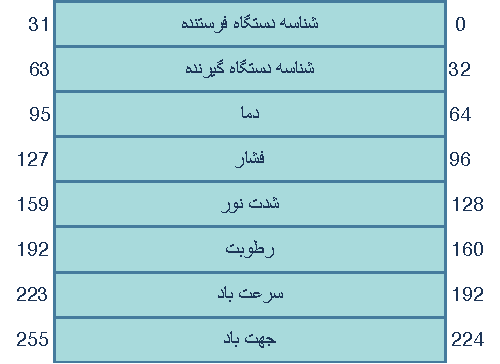
\includegraphics[width=0.6\linewidth]{Assets/sensorData.pdf}
	\caption{ساختار داده‌ها پس از تبدیل به ساختار اصلی در سمت ایستگاه.}
	\label{fig:sensorDataConverted}
\end{figure}

پس از این تبدیل شناسه دستگاه گیرنده که در دومین جایگاه آرایه داده‌های تبدیل شده قرار دارد با شناسه ثبت شده در دستگاه سمت ایستگاه بررسی شده و در صورتی که با یکدیگر مطابقت داشتند داده‌های دریافت شده از طریق \متن‌لاتین{USB} به رایانه ارسال می‌شوند.

\زیرقسمت{نحوه ارسال اطلاعات از طریق USB}
از ‌انجایی که در این پروژه ار کتابخانه \متن‌لاتین{HAL} استفاده می‌کنیم فعال کردن واحد \متن‌لاتین{USB} به سادگی همانند فعال کردن بخش‌های \متن‌لاتین{I2C} و \متن‌لاتین{SPI} از طریق نر‌م‌افزار \متن‌لاتین{STM32CubeMX} قابل انجام است. برای این کار کافیست تیک \متن‌لاتین{Device} در قسمت \متن‌لاتین{USB} زده شود و سرعت یو اس بی مشخص شود. تصویر این تنظیمات در شکل \رجوع{fig:usb} قابل مشاهده است. پس از آن لازم است کلاس یو اس بی را مشخص کنیم. برای این کار تنها لازم است از قسمت \متن‌لاتین{Middleware} به قسمت \متن‌لاتین{USB\_Device} رفته و در قسمت \متن‌لاتین{Class for FS IP} کلاس مورد نظر خود را انتخاب کنیم. تفاوت و کاربر هر یک از این کلاس‌ها در بخش \رجوع{sec:usb} توضیح داده شده‌است. در اینجا ما قصد استفاده از کلاس \متن‌لاتین{CDC} یا \متن‌لاتین{Communication Device Class} را داریم. در این حالت (کلاس \متن‌لاتین{CDC} و یو‌اس‌بی فول اسپید) میتوانیم دیتا‌های بالک 64 بایتی را از طریق \متن‌لاتین{USB} مخابره کنیم. تصویر تنظیمات بخش کلاس در شکل \رجوع{fig:usb_device} آمده است. در این قسمت لازم است مقادیر \متن‌لاتین{VID} و \متن‌لاتین{PID} را مقادیری یکتا و مختص این نوع دستگاه وارد کنیم. مقدار \متن‌لاتین{VID} شناسه سازنده و مقدار \متن‌لاتین{PID} شناسه این نوع دستگاه است. در هنگام ثبت محصول به عنوان محصول نهایی و قابل عرضه در بازار لازم است عملکرد یو‌اس‌بی دستگاه مورد آزمایش واقع شده و با پس از دریافت گواهینامه‌های معتبر امکان خرید شناسه برای دستگاه میسر خواهد بود. البته شرکت‌هایی نیز هستند که میتوان از آن‌ها \متن‌لاتین{PID} دریافت کرد ولی در این صورت باید از \متن‌لاتین{VID}ای که به نام آن شرکت است استفاده نمود. برای تست و توسعه می‌توان هر مقدار \متن‌لاتین{PID} و \متن‌لاتین{VID}‌ای که توسط دستگاه‌های متصل به رایانه خود استفاده نمی‌شود استفاده کرد. مقادیر \متن‌لاتین{Manufacture String} و \متن‌لاتین{Product String} نیز مقادیری هستند که در صورت اتصال دستگاه به رایانه به عنوان نام سازنده دستگاه و نم دستگاه نمایش داده می‌شود.

\begin{figure}[H]
	\centering
	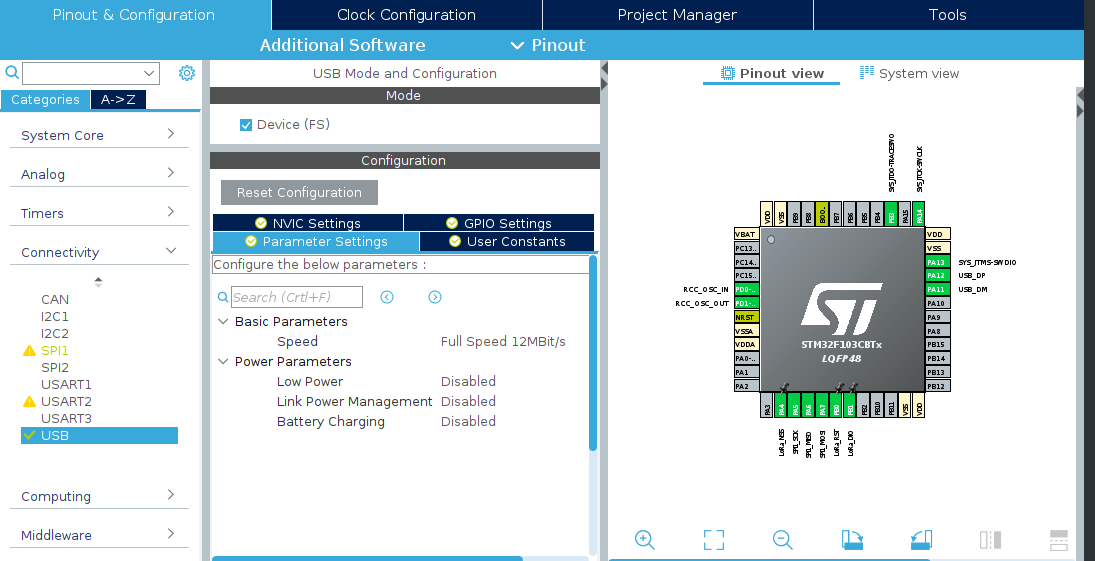
\includegraphics[width=\linewidth]{Assets/usb.png}
	\caption{تنظیمات \متن‌لاتین{USB} در نرمافزار \متن‌لاتین{STM32CubeMX}.}
	\label{fig:usb}
\end{figure}

\begin{figure}[H]
	\centering
	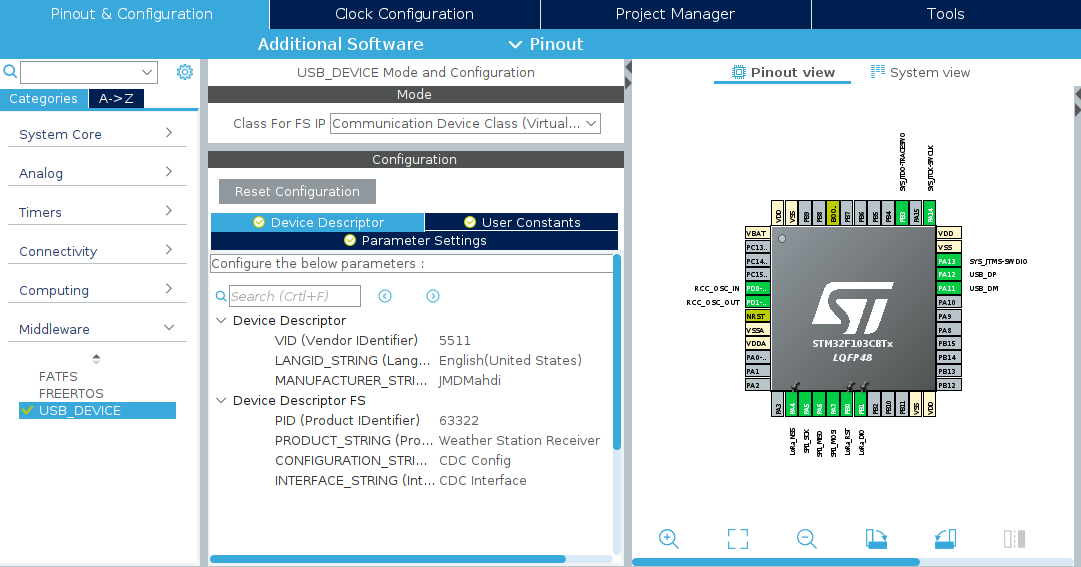
\includegraphics[width=\linewidth]{Assets/usb_device.png}
	\caption{تنظیمات \متن‌لاتین{USB\_Device}  در نرمافزار \متن‌لاتین{STM32CubeMX}.}
	\label{fig:usb_device}
\end{figure}

جهت ارسال داده‌ها از طریق کتابخانه \متن‌لاتین{HAL}، به سادگی می‌توان از دستور \متن‌لاتین{CDC\_Transmit\_FS} استفاده کرد. این دستور دو پارامتر داده‌ ارسالی و سایز داده را دریافت کرده و داده را از طریق \متن‌لاتین{USB} به دستگاه \متن‌لاتین{Host} مخابره می‌کند. نوع داده‌های دریافتی در این قسمت نیز همانند داده‌های دریافتی در ماژول لورا آرایه‌ای از داده‌های 8 بیتی بدون علامت است. پس میتوان همان داده‌های دریافت شده از طریق لورا را نیز مستقیما از طریق همین دستور و بدون هیچ تبدیل اضافه از طریق \متن‌لاتین{USB} به رایانه ارسال کرد. این تابع به طور خودکار در صورتی که سایز داده‌های ارسالی بیشتر از 64 بایت باشد داده ارسالی را به چندین بسته بالک 64 بایتی تقسیم می‌کند. در اینجا ما 32 بایت داده را از لورا دریافت می‌کنیم و دقیقا همان داده‌ها را میخواهیم ارسال کنیم پس داده‌ها در یک بسته بالک به خوبی جای می‌گیرند. تصویر این داده‌های در شکل \رجوع{fig:loraDataReceive} در بخش‌های قبلی آمده است.

\زیرقسمت{حالت خواب میکروکنترلر}
داده‌های ارسالی ار طریق ماژول لورا در سمت سنسور هر سه ساعت یک بار ارسال می‌شوند و در سمت سنسور نیز ان داده‌ها در سه ساعت یک‌بار دریافت می‌شوند به همین جهت و دقیقا مشابه سمت سنسور به دلیل تمایل به ذخیره انرژی در بین این ساعات بی‌کاری میکروکنترلر را در حالت خواب قرار می‌دهیم. تفاوت حالت خواب با حالت توقف که در سمت سنسور از آن استفاده کردیم در این است که در این حالت میکروکنترلر می‌تواند با هریک از \متن‌لاتین{peripheral}‌های فعال از خواب برحیزد و به کار خود ادامه دهد و پس از اتمام کار دوباره به خواب برود. در این سمت به دلیل استفاده از یو‌اس‌بی از این مود استفاده کردیه‌ایم تا در صورت رخ دادن هر گونه خطای سخت افزاری در اتصالات و یا ریست‌های نرم افزاری در سمت هاست پس از رفع و ثابت شدن وضعیت مجبور به قطع و وصل کردن کابل یو اس بی متصل به دستگاه نباشم. 

در این حالت مصرف میکروکنترلر چیزی در حدود 400 میکروآمپر خواهد بود. البته که ماژول لورا در این حالت در مود دریافت بدون وقفه خود قرار دارد و در صورت دریافت اطلاعات جدید میکروکنترلر را با اعمال اینتراپت خارجی از خواب بیدار می‌کند تا دیتای دریافت شده را گرفته و از طریق یو اس بی به رایانه منتقل نماید. 

\قسمت{برنامه دسکتاپ}
برنامه دسکتاپ که با زبان \متن‌لاتین{Python} نوشته شده است، متشکل از سه بخش \متن‌لاتین{Home}، \متن‌لاتین{Charts} و \متن‌لاتین{Log} می‌باشد. در بخش \متن‌لاتین{Home} اطلاعات آخرین دیتای دریافت شده به نمایش درمی‌آید. در بخش \متن‌لاتین{Charts} نمودارهای دیتاهای دریافتی در بازه قابل‌تعیین توسط کاربر به نمایش درمی‌آید. تمام رخدادهایی که در ارتباط با دستگاه رخ می‌دهد نظیر دریافت دیتای جدید و یا اتصال یا قطع اتصال دستگاه در تب \متن‌لاتین{Log} با ذکر زمان لیست می‌شوند. 

\begin{figure}[H]
	\centering
	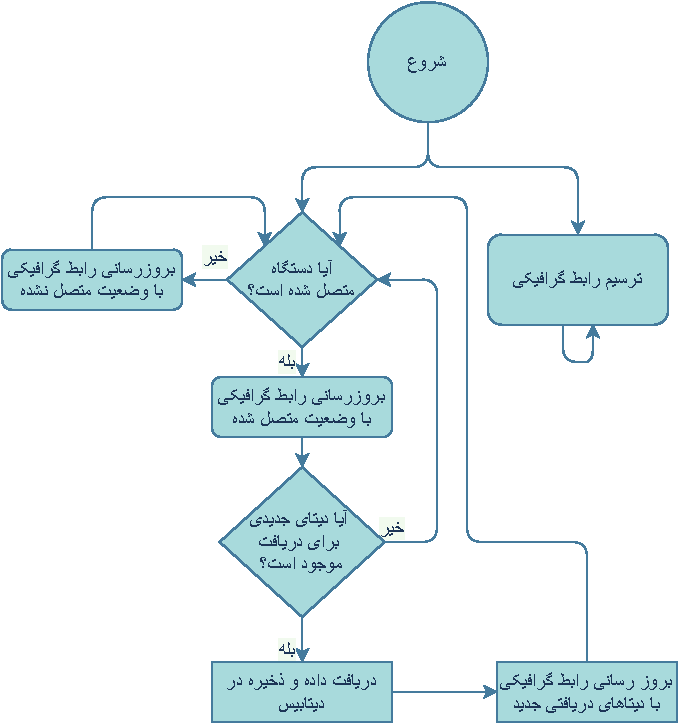
\includegraphics[width=0.7\linewidth]{Assets/USBFlowChart.pdf}
	\caption{فلوچارت برنامه دسکتاپ.}
	\label{fig:USBFlowChart}
\end{figure}

فلوچارت برنامه دسکتاپ در شکل \متن‌لاتین{fig:USBFlowChart} آمده است. نحوه عملکرد برنامه دسکتاپ به شرح زیر است:

\شروع{فقرات}
\فقره
با اجرای برنامه \متن‌لاتین{Thread} اصلی وظیفه ترسیم رابط گرافیکی برنامه\پانویس{Graphical user interface (GUI)}، که با \متن‌لاتین{PyQt5} پیاده‌سازی شده است، را برعهده می‌گیرد.
\فقره 
در همین حین \متن‌لاتین{Thread} دیگر به کمک کتابخانه \متن‌لاتین{libusb} مسئول بررسی وضعیت اتصال دستگاه به رایانه و دریافت اطلاعات ارسالی از دستگاه می‌شود.
\فقره 
در صورت تغییر وضعیت اتصال و یا دریافت اطلاعات، مشخصات آن در تب \متن‌لاتین{Log} ثبت می‌شود و برای کاربر قابل‌مشاهده خواهد بود.
\فقره
هنگام دریافت اطلاعات جدید از طریق \متن‌لاتین{USB} علاوه بر نمایش در تب اصلی برنامه، به‌روزرسانی تب \متن‌لاتین{Charts} با اطلاعات جدید و ثبت رخ داد در تب \متن‌لاتین{Log}، مشخصات کامل آن در دیتابیس \متن‌لاتین{SQLite} در کنار فایل اجرایی برنامه نیز ذخیره می‌شود. 
\فقره 
در تب \متن‌لاتین{Charts} با انتخاب بازه زمانی، نمودارها باتوجه به اطلاعات ثبت‌شده آن بازه زمانی در دیتابیس بروز می‌شوند.
\پایان{فقرات}

\زیرقسمت{نحوه طراحی رابط کاربری}
از برنامه \متن‌لاتین{Qt Designer} برای طراحی محیط \متن‌لاتین{GUI} برنامه استفاده شده است که تصویری از محیط این نرم افزار را در شکل \رجوع{fig:qtDesigner} مشاهده می‌کنید. در این برنامه به راحتی با درگ و دراپ کردن ویجت‌ها در بخش‌های مورد نظر میتوان رابط کاربری برنامه خود را ساخت. در پنل سمت راست این برنامه نیز می‌توان جزئیات بیشتری از هر ویجت را دید و به تنظیمات بیشتری دسترسی داشت. 

\begin{figure}[!h]
	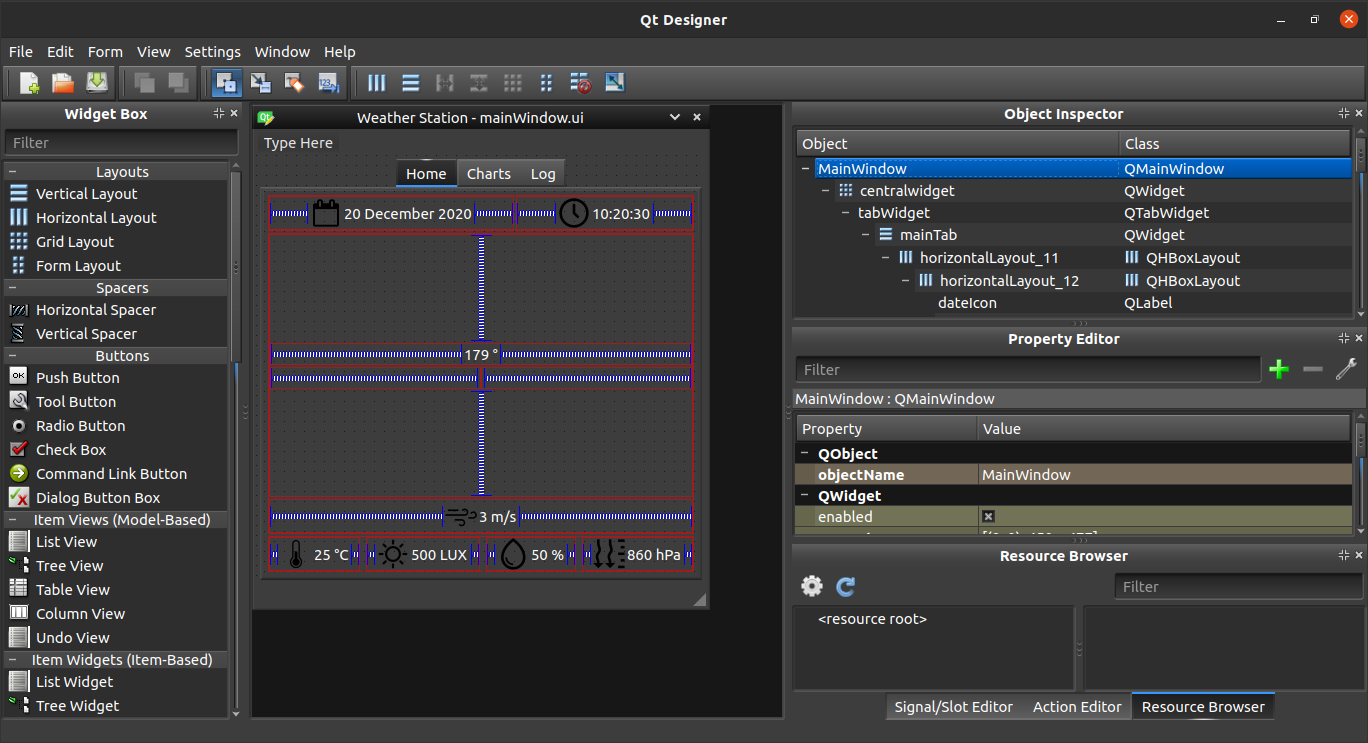
\includegraphics[width=\linewidth]{Assets/qtDesigner.png}
	\caption{طراحی محیط برنامه با نرم افزار \متن‌لاتین{Qt Designer}.}
	\label{fig:qtDesigner}
\end{figure}

برای این برنامه یک ویجت از نوع \متن‌لاتین{tabWidget} با 3 تب اضافه می‌کنیم. این تب‌ها همان سه بخش اصلی برنامه یعنی \متن‌لاتین{Home}، \متن‌لاتین{Charts} و \متن‌لاتین{Log} را در بر می‌گیرند. در این صورت با کلیک کردن روی هر تب اطلاعات موجود در آن تب را نشان می‌دهند.  

حهت نمایش چارت‌ها در تب \متن‌لاتین{Charts} از ویجتی با عنوان \متن‌لاتین{chartWidget} استفاده می‌کنیم. برای افزودن اطلاعات به این نمودار‌ها از سری‌هایی از نوع \متن‌لاتین{QLineSeries} استفاده می‌کنیم. محور افقی این نمودار‌ها را زمان ثبت شدن دیتا‌ها در دیتابیس و محور عموی را مقدار داده‌های ذخیره شده در دیتابیس در نظر می‌گیریم. برای هر یک از داده‌های دما، رطوبت، فشار، سرعت باد، جهت باد و شدت نور نموداری از همین نوع و مستفل رسم می‌کنیم. در بالای نمودار‌ها دو ویجت از نوع \متن‌لاتین{datePicker} قرار داده شده است که کاربر با انتخاب آن میتواند تاریخ شروع و پایان را مشخص کند با مشخص کردن تاریخ شروع و پایان داده‌های نمودار‌ها با اطلاعات متناظر با بازه انتخابی بروز می‌شوند. در اینجا تفاوتی ندارد که در کدام باکس تاریخ شروع و در کدام باکس تاریخ پایان را وارد کند برنامه طوری نوشته شده است که به طور خودکار تاریخی که از دیگری کوچک تر است را به عنوان تاریخ شروع و تاریخ دیگر را به عنوان تاریخ پایان در نظر بگیرد. همچنین به دلیل اینکه ارتفاع این نمودار‌ها زیاد است آن‌ها را در ویجتی از نوع \متن‌لاتین{scrollArea} قرار داده‌ایم تا امکان اسکرول کردن به این تب اضافه شود. 

در تب \متن‌لاتین{Log} یک ویچت از نوع چک باکس و پایین آن یک ویجت از نوع \متن‌لاتین{textBrowser} قرار داده شده است. لاگ‌های رخ داد‌های برنامه نظیر قطع و وصل دستگاه، دریافت اضلاعات جدید و وضعیت افزودن دیتا‌ها به دیتابیس در این قسمت با زمان دقیق رخ داد لیست خواهند شد. همچنین در صورتی که تیک چک باکس بالای باکس متنی زده شده باشد در صورت افزوده شدن ردیف‌های متنی جدید اسکرول بار باکس متن به آخرین خط اضافه شده منتقل می‌شود و در غیر این صورت (در صورتی که چک‌باکس تیک زده نشده باشد) اسکرول باکس متنی تغییری نخواد کرد.  


\زیرقسمت{ساختار دیتابیس}
به جهت ذخیره داده‌های از دیتابیس \متن‌لاتین{SQLite} استفاده می‌کنیم. دلیل این امر پشتیبانی اکثر زبان‌ها و سیستم عامل‌ها از این نوع دیتابیس و سادگی و قابل حمل بودن آن است. ساختار جدول دیتابیس \متن‌لاتین{SQLite}ای که اطلاعات پس از دریافت از طریق \متن‌لاتین{USB} در آن ذخیره می‌شود در تصویر \رجوع{fig:DBStructure} آمده است.

\begin{figure}[!h]
	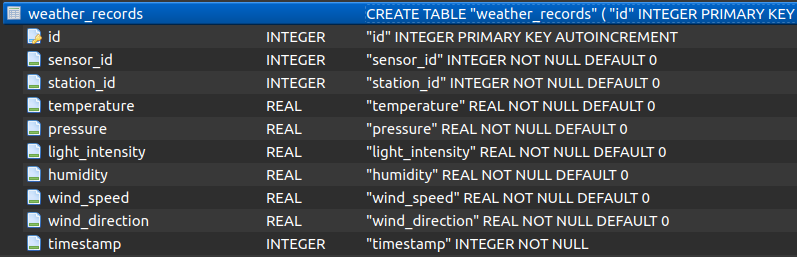
\includegraphics[width=\linewidth]{Assets/dbStructure.png}
	\caption{ساختار جدول دیتابیس.}
	\label{fig:DBStructure}
\end{figure}

در برنامه پس از اجرا در صورتی که فایل دیتابیس ویا جدول دیتابیس موجود نباشد فایل و جدول دیتابیس ساخته می‌شود. این فایل در کنار فایل اجرایی برنامه در پوشه \متن‌لاتین{DB} و با عنوان \متن‌لاتین{weatherStation.db} قرار می‌گیرد. این فایل را می‌توان به سادگی با نرم افزار‌های مدیریت دیتابیس \متن‌لاتین{Sqlite} باز کرد و دیتاهای ذخیره شده را ویرایش کرد و یا به سیستم‌ و دیتابیس‌های دیگر منتقل کرد. همچنین می‌توان با اکثر زبان‌های برنامه نویسی کوئری‌های مورد نظر را روی این فایل و دیتابیس به جهت دریافت یا ثبت داده‌ها اجرا کرد. 

پارامتر \متن‌لاتین{id} در این جدول پارامتری عددی صحیح و یکتا است که به طور خودکار با افزودن دیتا‌های جدید مقدار آن یک واحد افزایش می‌یابد. در این صورت هر دیتا ثبت شده علاوه بر زمان ثبت، که در پارامتر  \متن‌لاتین{timestamp} ثبت می‌شود، شناسه‌ای یکتا (\متن‌لاتین{id}) برای خود خواهند داشت. پارامتر \متن‌لاتین{timestamp} مقداری عددی صحیح می‌پذیرد و در آن مقدار ثانیه‌های گذشته از تاریخ مرجع \متن‌لاتین{Jan 01 1970} تا تاریخ مورد نظر قرار داده می‌شود. به این نوع نحوه ثبت زمان، که ثانیه‌های گذشته از تاریخ \متن‌لاتین{Jan 01 1970} تا تاریخ مورد نظر برای ثبت است، \متن‌لاتین{Unix Time} و یا \متن‌لاتین{Timestamp} گفته می‌شود. مابقی پارامتر‌ها مقادیر دریافت شده از \متن‌لاتین{USB} را درون خود جای می‌دهند و به دلیل اینکه نوع داده‌های دریافت شده \متن‌لاتین{float} بوده است این پارامترها مقادیری از توع اعداد حقیقی دارند که این نوع اعداد را می‌تواند بدون مشکل در خود جای دهد.

پس از اتمام طراحی این برنامه (\متن‌لاتین{Qt Designer}) خروجی‌ای با پسوند \متن‌لاتین{UI} به ما می‌دهد. این فایل را میتوانیم با ابزار‌های دیگری که در کنار این نرم افزار ارائه می‌شود به کد‌های قابل استفاده در زبان‌های برنامه نویسی قابل پشتیابنی تبدیل کرد. برای مثال برای تبدیل این فایل به کد‌های قابل استفاده در پایتون از دستور زیر استفاده می‌کنیم. 

\begin{latin}
	\noindent
	pyuic5 mainWindow.ui -o mainWindow.py
\end{latin}

\noindent
که با دریافت فایل \متن‌لاتین{mainWindow.ui} فایل خروجی \متن‌لاتین{mainWindow.py} را به ما تحویل می‌دهد که از آن می‌توانیم مستقیما در برنامه خود استفاده کنیم.

\زیرقسمت{نحوه دریافت اطلاعات از طریق \متن‌لاتین{USB}}
برای دریافت اطلاعات ارسال شده از سخت افزار سمت ایستگاه به رایانه لازم است در ابتدا رایانه کلاس دستگاه را بشناسد تا بتواند با آن به درستی ارتباط برقرار کند. برای کلاس \متن‌لاتین{CDC} استفاده شده بهترین درایور قابل استفاده که تمامی امکانات این کلاس را پوشش دهد درایور \متن‌لاتین{LibUSB} است. این درایور در سیستم‌های لینوکسی و مبتنی بر یونیکس به طور دیفالت روی سیستم موچود است و فقط کافیست دسترسی برنامه به یو اس بی از طریف تنظیمات \متن‌لاتین{udev} باز شود تا برنامه بتواند دستگاه متصل شده را دیده و با آن ارتباط برقرار کند. در محیط ویندوز این مسئله کمی متفاوت است و باید حتما به صورت جداگانه درایور \متن‌لاتین{LibUSB} برای این دستگاه نصب شود. از نرم افزار \متن‌لاتین{Zadig} می‌توان به این منظور استفاده کرد. تصویری از محیط این نرم افزار در هنگام نصب درایور در شکل \رجوع{fig:usbDriver} آمده است.

به جهت برنامه نویسی این قسمت از کتابخانه \متن‌لاتین{PyUSB} در زیان برنامه نویسی پایتون استفاده شده است. پس از افزودن این کتابخانه به پروژه لازم است در ابتدا بک‌اند این کتابخانه نیز مشخص گردد. بک‌اند این کتابخانه باید متناسب با ورژن درایور نصب شده انتخاب گردد. در سیستم‌عامل‌های مبتنی بر یونیکس به جهت وجود درایور \متن‌لاتین{LibUSB} این کار لازم نیست و به طور خودکار این کار توسط خود کتابخانه انجام می‌شود. 

\begin{figure}[!t]
	\centering
	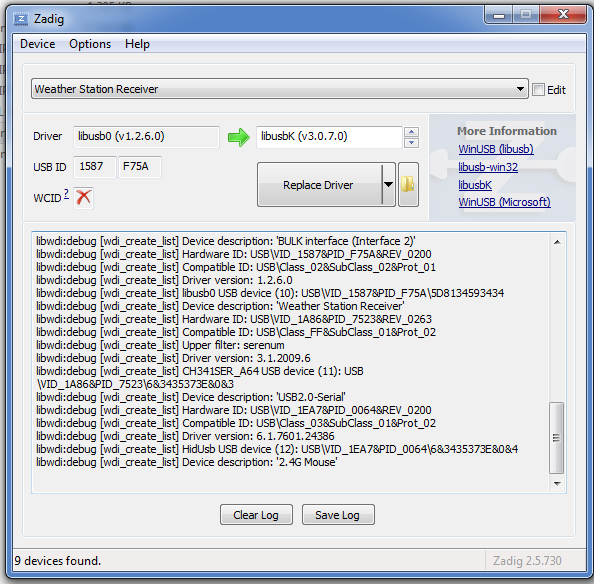
\includegraphics[width=0.7\linewidth]{Assets/usbDriver.png}
	\caption{تصویری از محیط نرم افزار نصب درایور \متن‌لاتین{Zadig}.}
	\label{fig:usbDriver}
\end{figure}

چک کردن وضعیت اتصال یو اس بی به دستگاه و یا دریافت اطلاعات باید در \متن‌لاتین{Thread} جدا از \متن‌لاتین{Thread} اصلی که مسئول ترسیم رابط گرافیکی برنامه است انجام شود. در غیر ان صورت در هنگام انجام فرآیند‌های چک کردن وضعیت و دریافت اطلاعات رابط کاربری برنامه قفل شده و امکان کلیک کردن روی دکمه‌ها و رفتن به بخش‌های دیگر برنامه ممکن نیست. تمامی فرآیند‌های چک کردن ارتباط با دستگاه و دریافت اطلاعات از آن با استفاده از کتابخانه \متن‌لاتین{PyUSB} انجام می‌شود.

اطلاعاتی که در این بخش دریافت می‌شود اطلاعاتی از نوع \متن‌لاتین{bytearray} و یا \متن‌لاتین{Uint8Array} هستند که ساختار تصویر \رجوع{fig:USBDataReceive} را دارند (که همان ساختار ارسال شده از طرق لورا است). برای دست‌یابی به دیتا‌های اولیه لازم است این داده‌ها را به لیستی از اعداد \متن‌لاتین{float} 32 بیتی تبدیل کنیم. این کار با کنار هم قرار دادن هر 4 بایت از این داده‌ها میسر می‌شود. برای این کار از کتابخونه \متن‌لاتین{numpy} و توابعی که به همین منظور دارد استفاده می‌کنیم تا درنهایت به ساختار تصویر \رجوع{fig:USBDataConverted} برسیم.  

\begin{figure}[H]
	\centering
	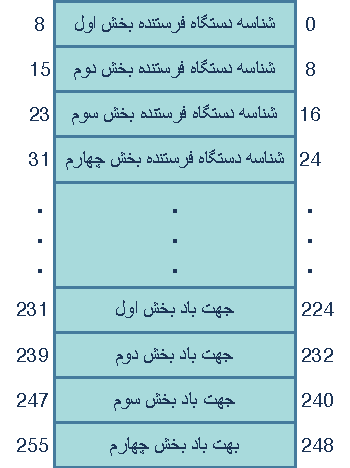
\includegraphics[width=0.4\linewidth]{Assets/loraData.pdf}
	\caption{ساختار داده‌های دریافت شده از طریق \متن‌لاتین{USB}.}
	\label{fig:USBDataReceive}
\end{figure}

\begin{figure}[H]
	\centering
	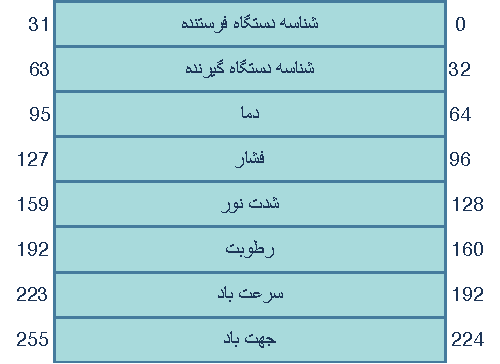
\includegraphics[width=0.6\linewidth]{Assets/sensorData.pdf}
	\caption{ساختار داده‌ها پس از تبدیل به ساختار اصلی در برنامه دسکتاپ.}
	\label{fig:USBDataConverted}
\end{figure}

در این صورت ساختاری مشابه ساختار اطلاعات جمع آوری شده در سمت سنسور را داریم که دقیقا با همان اطلاعات جمع آوری شده پر شده است و میتوانیم مستقیما با دسترسی به خانه‌های مختلف آن مقادیر مورد نظر را گرفته و در دیتابیس برای استفاده‌های بعدی ذخیره کنیم.
